\chapter{SISTEMA PRODUTIVO}
\label{chap:sistemas_produtivos}

\section{Medidas de desempenho} 
\label{sec:sistemas_produtivos_desempenho} 
Para medir o desempenho de uma operação produtiva é necessário o uso de indicadores para isso foi criado um sistema chamado de \textit{Balanced Scorecard (BSC)}, este é utilizado por ser considerado o mais equilibrado na aferição dos indicadores de desempenho da operação.
Na Figura \ref{fig:balanced_scorecard} tem-se uma versão adaptada do BSC, e os indicadores são os seguintes:

\begin{itemize}
    \item Indicadores financeiros, de particular interesse para os acionistas e proprietários do negócio;
    \item Indicadores da percepção do cliente sobre os produtos e sobre o negócio, os quais se traduzem em decisões de compra;
    \item Indicadores dos processos internos da operação, os quais são comparados com os parâmetros operacionais a serem observados;
    \item Indicadores de aprendizagem e crescimento, que refletem a habilidade que a operação tem para aprender, mudar e melhorar, a fim de manter-se sustentável ao longo do tempo.  
\end{itemize}


\begin{figure}[H]
    \caption{Balanced Scorecard (BSC)}
    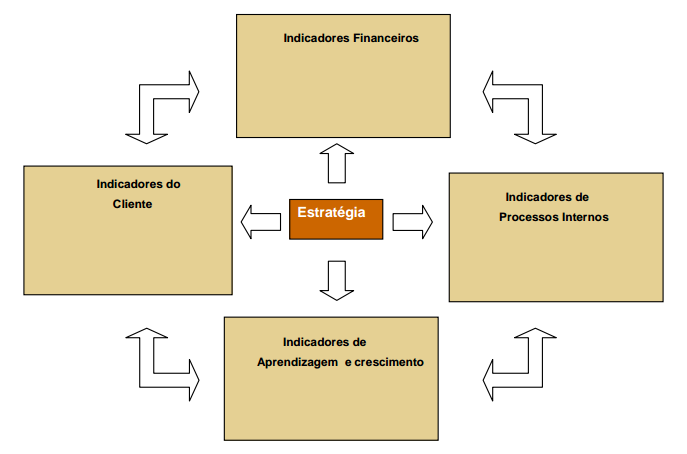
\includegraphics[width =\textwidth]{images/bsc.png}
    \caption*{Fonte: Adaptado de \cite{kaplan1996using}}
    \label{fig:balanced_scorecard}
\end{figure}
  

\section{Aplicação Prática} 
\label{sec:estrategia_da_producao_aplicacao}





